% vim:syntax=tex

In this section we describe how a topic model-based feature location
technique can use changesets.



\begin{figure*}
\vspace{2mm}
\centerline{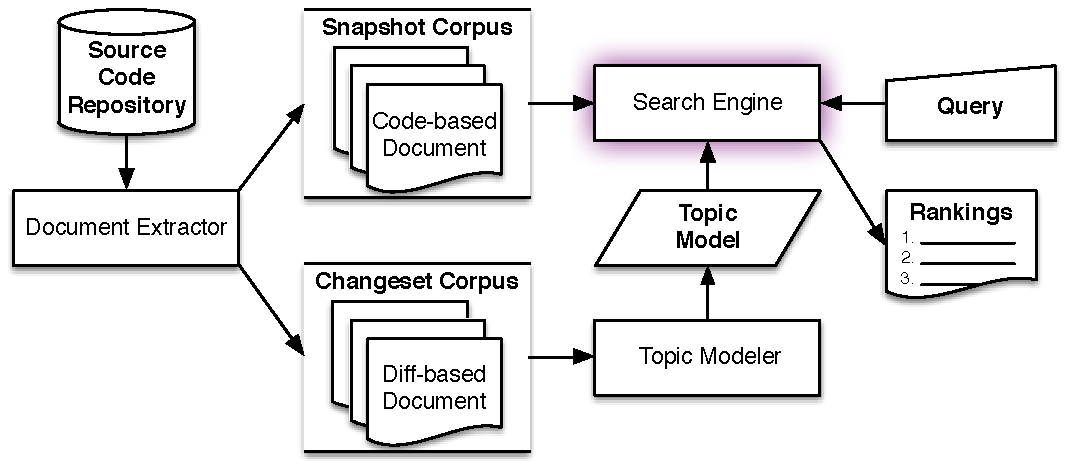
\includegraphics[width=.75\textwidth]{figures/changeset-flt}}
\caption{Feature location using changesets}
\label{fig:changeset}
\vspace{-2mm}
\end{figure*}

We use the following terminology to describe document extraction of changesets.
A \textit{diff} is a set of text which represents the differences between two texts.
A \textit{patch} is a set of instructions (i.e., diffs) that is used to transform one set of texts into another.
\textit{Context lines} denote text useful for transforming the text, but do not represent the differences.
\textit{Added lines} are lines which were added in order to transform the first text into the second.
Similarly, \textit{removed lines} are lines which are removed for this same purpose.
Figure~\ref{fig:diff} shows an example of what a changeset might look like.
A \textit{changeset}, ideally, represents a single feature modification,
addition, or deletion, which may crosscut many source code entities.
A \textit{commit} is a representation of a changeset in a version control system.
The terms changeset and commit are often used interchangeably.

The document extraction process for changesets remains mostly the same as covered in Section~\ref{sec:related}.
However, instead of extracting documents by parsing source code for identifiers, comments, and literals,
the changeset itself is parsed.
In a changeset it may be desirable to parse further for source code entities using island grammar parsing\needcite.
The same preprocessor transformations may also occur in changesets.

To leverage the online functionality of the topic models,
we intermix the model training and retrieval steps.
First, we initialize a model in online mode.
Then, as changes are made, the model is updated with the new changesets as they are committed.
That is, with changesets, we incrementally update a model and can query it at any moment.

We can use a dynamic programming to keep a separate $\theta_{snapshot}$
up-to-date as new changesets are added to the model.
That is, upon a update to the model, new inferences of on only the source code documents affected by this changeset are made.
Additionally, we can then query the model as needed
and rank the results of that query against $\theta_{snapshot}$.
Note that we never care about infering a $\theta_{changeset}$
for the changeset documents on which the model is built.


%diff --git a/lao b/tzu
%index 635ef2c..5af88a8 100644
%--- a/lao
%+++ b/tzu
\begin{figure}[t]
\centering
\footnotesize
\begin{lstlisting}[language=diff, basicstyle=\ttfamily]
--- lao
+++ tzu
@@ -1,7 +1,6 @@
-The Way that can be told of is not the eternal Way;
-The name that can be named is not the eternal name.
 The Nameless is the origin of Heaven and Earth;
-The Named is the mother of all things.
+The named is the mother of all things.
+
 Therefore let there always be non-being,
   so we may see their subtlety,
 And let there always be being,
@@ -9,3 +8,6 @@ And let there always be being,
 The two are the same,
 But after they are produced,
   they have different names.
+They both may be called deep and profound.
+Deeper and more profound,
+The door of all subtleties!
\end{lstlisting}
\caption{Example of a \texttt{git diff}.
Black or blue lines denote metadata about the change useful for patching.
In particular, black lines represent context lines (beginning with a single space).
Red lines (beginning with a single~\texttt{-}) denote line removals,
and green lines (beginning with a single~\texttt{+}) denote line additions.}
\label{fig:diff}
\vspace{-10pt}
\end{figure}
